\documentclass[licencjacka,openright]{pracamgr}
\usepackage{latexsym}
\usepackage[MeX]{polski}
\usepackage[utf8]{inputenc}
\usepackage{graphicx}
%\usepackage{afterpage}
\usepackage{rotating}
%\usepackage{subfigure}%
\usepackage{polski}
\usepackage{natbib}
\usepackage{indentfirst}
\usepackage{graphicx}
\usepackage{url}
\usepackage{float}
\usepackage{amsmath}
\usepackage{antpolt}
\usepackage[T1]{fontenc}
\usepackage[draft]{todonotes}
\usepackage{hyperref}
\usepackage{booktabs}
\usepackage{chngcntr}


\author{ Karol Auguštin }
\nralbumu{ 249476 }
\title{ Filtry przestrzenne w detekcji potencjału P300 }
\tytulang{ Spatial filters in detection of P300 evoked potential }
\kierunek{Zastosowania fizyki w biologii i medycynie}
\opiekun{dr hab. Jarosława Żygierewicza \\ Zakład Fizyki Biomedycznej \\ Instytut Fizyki Doświadczalnej \\ Uniwersytet Warszawski}
\dziedzina{13.2}
\specjalnosc{Neuroinformatyka}
\date{Warszawa, Wrzesień 2013}
\keywords{P300, filtry przestrzenne, interfejsy mózg -- komputer, CSP} 

%\bibliographystyle{elsart-harv}
\bibliographystyle{unsrt}

\begin{document}
\let\cleardoublepage\clearpage
\maketitle
\begin{abstract}
\par Streszczenie
\end{abstract}
\tableofcontents
%\addcontentsline{toc}{chapter}{Cel pracy}

\chapter{Wstęp}
\section{Diagnostyka medyczna}
\todo[inline]{dopisać co to sa potencjaly, orientacja w czasie i przestrzeni}
Istnieje wiele udokumentowanych zastosowań detekcji potencjału P300 w~diagnostyce medycznej chorób układu nerwowego, zaburzeń psychicznych, a~także uszkodzeń mózgu w~wyniku urazów \cite{zgorzalewicz2000}.\todo[inline]{nie wiem czy dać ten format cytacji czy ten z nawiasami (Autor, rok)} Opierają się one głównie na analizie wielu cech rejestrowanego potencjału takich jak: latencja względem bodźca, kształt, oraz miejsce występowania na powierzchni czaszki. Praktycznie we~wszystkich przypadkach opisanych w~literaturze sposób badania jest identyczny, jeśli porównywany jest od strony analizy sygnału. Pacjentowi podawany jest wielokrotnie bodziec standardowy (ang. target), przeplatany z bodźcem celowym (ang. non-target), mającym wygenerować u pacjenta potencjał P300. Następnie przeprowadzane jest uśrednianie wystąpień bodźca celowego dla każdej z~elektrod i~analiza takiego wyniku wykonywana przez lekarza. 
W związku z~tym, że~najistotniejszym elementem badania diagnostycznego jest amplituda oraz czas wystąpienia reakcji, jak również umiejscowienie jej na~powierzchni czaszki \todo[noline]{cite} jedynymi powszechnie stosowanymi metodami analizy sygnałów są~filtrowanie pasmowe i~uśrednianie, natomiast nie jest praktykowane użycie filtrów przestrzennych, czy innych metod mających na celu lepsze uwidocznienie potencjału.
\section{Interfejsy mózg -- komputer}
Najbardziej obiecującym zastosowaniem zautomatyzowanej analizy sygnału EEG są~obecnie interfejsy mózg-komputer (brain-computer interface -- BCI) mające na~celu umożliwienie komunikacji użytkownika z~komputerem bez użycia mięśni jedynie lub głównie poprzez analizę sygnału EEG zbieranego z powierzchni czaszki użytkownika. Aby umożliwić wykorzystanie potencjału P300 w~takim zastosowaniu potrzebny jest złożony z~wielu elementów aparat matematyczno -- informatyczny, za~pomocą którego w~zautomatyzowany sposób można by rejestrować wystąpienie w pojedynczej lub niewielkiej ilości realizacji potencjałów P300 w~sposób nie~wymagający udziału przeszkolonej osoby. Jako, że~w~takiej sytuacji istotny jest nie kształt czy opóźnienie załamka P300, a~samo jego wystąpienie w~reakcji na~określony bodziec dostępne są~wszystkie metody cyfrowej analizy sygnałów, o~ile okażą się~skuteczne.
\subsection{Dostęp do informacji}
Od lat osiemdziesiątych mamy do~czynienia z~dynamicznym rozwojem informatyzacji społeczeństwa, nie~tylko w~warstwie możliwości technicznych, ale~przede wszystkim w~rozumieniu społecznym. Przez ostatnie trzydzieści lat stopień zastosowania komputerów i~urządzeń elektronicznych przez społeczeństwo wzrósł, a~co~ważniejsze wzrost ten nadal występuje w~olbrzymim tempie. Unowocześnianie i~ułatwianie ludziom dostępu do~komputerów i~możliwości jakie ten dostęp umożliwia jest kluczowym zadanie producentów i~projektantów wszystkich firm produkujących urządzenia elektroniczne przeznaczone dla masowego odbiorcy. Sposób komunikacji użytkowników z~komputerem ewoluował na przestrzeni lat. Od klawiatury podłączonej do~terminala tekstowego w~latach osiemdziesiątych przez wprowadzenie na~rynek myszki i~interfejsu graficznego przez firmę Apple Computers Inc. w~1984 roku, aż~do~obecnie znanych i~coraz szerzej stosowanych ekranów dotykowych. Historia komunikacji człowieka z urządzeniami elektronicznymi pokazuje jak istotny dla współczesnego świata jest sposób dostępu człowieka do możliwości jakie dają współczesne komputery.

Rozwój urządzeń umożliwiających komunikację ludzi z~komputerami opiera się na~stosowaniu technologii eliminujących nienaturalnych i~zbędnych urządzeń pośredniczących w tejże komunikacji. Najpierw ograniczono rolę klawiatury, na~rzecz dużo prostszej i~bardziej naturalnej myszki, żeby w końcu i~z~niej zrezygnować na rzecz ekranu obsługiwanego w naturalny dla człowieka sposób -- palcami. Kolejnym krokiem w~tej ewolucji jest wyeliminowanie konieczności używania jakiegokolwiek urządzenia obsługiwanego za pomocą mięśni na rzecz bezpośredniego połączenia komputera z~mózgiem użytkownika.

%Rozwój metod rejestracji i~analizy sygnału EEG daje nadzieję, że w~przyszłości będzie to możliwe i~dostępne dla zwykłego użytkownika.
\subsection{Pomoc osobom niepełnosprawnym}
Kolejnym aspektem zastosowania systemów BCI w~postaci, w~jakiej istnieją one dzisiaj jest pomoc osobom niepełnosprawnym, w~szczególności sparaliżowanym, pozbawionym możliwości kontaktu ze~światem zewnętrznym za pośrednictwem mięśni. Urządzenia BCI Appliance tworzone i~rozwijane na~wydziale Fizyki Uniwersytetu Warszawskiego już dzisiaj dają taką możliwość.
\todo{Inne bci + cite}
Opierając się na znanych mechanizmach działania mózgu umożliwiają wprowadzanie informacji do komputera jedynie za pomocą analizy sygnału EEG związanego z koncentracją uwagi na określonych bodźcach. Jednym z paradygmatów, na którym opiera się ten system jest właśnie rejestracja i~analiza potencjału P300.

\section{Cel pracy}
%I będzie w nim napisane że zbadasz i zaprezentujesz jak zastosowanie różnych filtrów przestrzennych wpływa na możliwość wykrywania wystąpienia P300, co przyczynia się do konstrukcji lepszych BCI opartych o P300.

Celem pracy jest zbadanie oraz zaprezentowanie jak~zastosowanie filtrów przestrzennych wpływa na~możliwość wykrywania występowania potencjału P300. Przyczynia się to do konstrukcji lepszych BCI opartych o paradygmat P300.

\chapter{Metodologia}
Potencjał P300 występujący w~sygnale EEG w~reakcji na~oczekiwany przez pacjenta bodziec ma złożoną charakterystykę, czyniąc go trudnym do automatycznej detekcji. Podstawowym problemem jest mała amplituda zjawiska na tle innych aktywności mózgu widocznych w sygnale EEG oraz duża zmienność osobnicza i zależność od wielu czynników zewnętrznych. \todo{cite + jakie}
Jedyną metodą uzyskania widocznego gołym okiem potencjału bez stosowania skomplikowanego aparatu matematycznego jest uśrednienie wielu realizacji eksperymentu. W takim przypadku aktywność mózgu nie związana z~występowaniem interesującego nas zjawiska jest modelowana jako szum nieskorelowany o~średniej zero, zatem ulega uśrednieniu do zera, a~interesująca nas, powtarzająca się dla każdej realizacji aktywność staje się widoczna. Takie podejście, poprawne w przypadku diagnostyki medycznej, niestety nie jest możliwe do~zastosowania w~systemach BCI, gdyż obniżyłoby skuteczność takiego systemu wymuszając na użytkowniku wielokrotne powtarzanie tej samej decyzji. Niski stosunek sygnału do szumu dla potencjału P300 bardzo utrudnia jego wykrycie przy użyciu jednej realizacji. Aby zminimalizować ilość niezbędnych powtórzeń występowania bodźca zaczęto stosować różnego rodzaju metody mające na celu wyeksponowanie go z szumu pozostałych aktywności mózgu, nie związanych z bodźcem podawanym pacjentowi.\todo{cite do prac o p300-bci}

%Zadanie jest tym trudniejsze gdyż charakterystyka odpowiedzi, jak również czas jej występowania po podaniu bodźca różni się pomiędzy pacjentami. 
Do najprostszych metod stosowanych w pierwszej kolejności należą przede wszystkim filtrowanie dolnoprzepustowe. \todo{tu dopiszę}

Bardziej zaawansowanymi metodami jest zaprojektowanie odpowiednich filtrów przestrzennych, mających na celu poprawę stosunku sygnału do szumu korzystając z~różnicy w rozkładzie przestrzennym szumu i~interesującej nas aktywności. Przykłady takich filtrów zostaną przedstawione w~kolejnych paragrafach.

\section{Filtry przestrzenne}
Filtry przestrzenne poprawiają stosunek sygnału do szumu wykorzystując różny rozkład przestrzenny składowej będącej sygnałem i~składowej będącej szumem, czyli sygnałem nie~zawierającym składowych istotnych z punktu widzenia badanego zagadnienia.
Filltr przestrzenny może być zrealizowany w postaci macierzy $M$ takiej,~że: 
Y = M*X
gdzie: $X$ oznacza sygnał mierzony, natomiast $Y$ sygnał filtrowany.

\subsection{Filtr tożsamościowy}
Aby zaobserwować efekty uzyskane za~pomocą różnych filtrów przestrzennych przedstawię dane zarejestrowane podczas eksperymentów bez użycia żadnego z~nich. Macierz przejścia dla takich danych jest macierzą, która na diagonali ma~wartości~1~oraz~0~w~pozostałych polach.
Dla trzech kanałów taka macierz ma~postać:
\[
M =
\begin{bmatrix}
  $1$ & $0$ & $0$ \\
  $0$ & $1$ & $0$ \\
  $0$ & $0$ & $1$ 
\end{bmatrix}
\]

\subsection{Transformata Hjorta}
Transformacja Hjortha \citep{hjorth1975} jest numerycznym przybliżeniem transformaty Laplace'a czyli drugiej pochodnej przestrzennej. Uzyskuje się ją poprzez odjęcie od każdego kanału średniej z kanałów go otaczających. Ma on na celu eliminację składowej wspólnej dla transformowanych kanałów, czyli pochodzącej od~źródeł odległych. Sygnał pozostający w~każdym kanale po zastosowaniu takiego filtra powinien odwzorowywać aktywność EEG zachodzącą bezpośrednio w~miejscu umieszczenia elektrody, eliminując czasem mocniejszą aktywność z~innych obszarów czaszki.
Macierz przejścia w~przypadku zastosowania takiego filtra jest ściśle związana z~lokalizacją elektrod na głowie pacjenta.
Transformacja ta ma postać przykładowo w~systemie EEG 10-20 dla elektrody $Cz$ ma~on~postać:
\begin{equation}
V'_{Cz} = V_{Cz} - 1/4(V_{Fz}+V_{C4}+V_{Pz}+V_{C4})
\end{equation}

\subsection{Wspólny wzorzec przestrzenny}
Wspólny wzorzec przestrzenny (ang. Common Spatail Patterns, CSP) \cite{koles1990} jest dyskryminacyjnym algorytmem pozyskującym przestrzenny filtr $W$ z~danych $X$, tak że różnica wariancji filtrowanego sygnału \mbox{$X_{CSP} = X \cdot W$} dla dwóch klas jest maksymalna w pewnym kanale $X_{CSP}$. Osiągane jest to poprzez jednoczesną diagonalizację macierzy kowariancji:\todo{cite}
\begin{equation}
\Sigma _2 W = (\Sigma _1 + \Sigma _2 )W \Delta
\end{equation}
gdzie $\Sigma_1$ i $\Sigma_2$ są kowariancjami macierzy sygnałów z~klas~1~oraz~2. Każda kolumna $W$ jest filtrem przestrzennym $w_i$ odpowiadającym wartości własnej $\delta _i$ w~macierzy $\Delta$, wartości $i = 1,2,3 \ldots N_c$ odpowiadają numerom kanałów sygnału oryginalnego.% \citep{sannelli2011}.

\section{Miara jakości}
\label{miara}
Jakość wstępnej analizy sygnałów jest tym lepsza im~zbiór cech wydobytych z~sygnału zarejestrowanego jako target jest różny od cech sygnału non-target będącego szumem z~punktu widzenia analizowanego zagadnienia.
%Jako, że zjawisko analizowane, takie jak wystąpienie potencjału P300, powtarzane jest w~każdej realizacji sygnału target, natomiast pozostałe zjawiska będące szumem nie są skorelowane z~bodźcem, uśrednienie wielu powtórzeń rejestracji pożądanego zjawiska powoduje wyeliminowanie sygnału pochodzącego od innych zjawisk na rzecz sygnału pochodzącego od zjawiska oczekiwanego.
%Jako, że czas wystąpienia potencjału P300 po podaniu bodźca jest powtarzalny dla danego pacjenta, proponowaną miarą jakości jest maksymalna wartość funkcji korelacji w otoczeniu zera pomiędzy średnią z~wszystkich sygnałów target uzyskanych podczas sesji kalibracyjnej oraz sygnałem poddawanym analizie.
%Miarą skuteczności danej metody jest odległość Mahalanobisa, zwana ważoną odległością euklidesową, którą można zastosować do mierzenia odległości pomiędzy dwoma zbiorami punktów~w przestrzeni wielowymiarowej.

Zgodnie z powszechnie używanym modelem potencjału wywołanego (sygnał deterministyczny + szum niezależny) proponowaną cechą  różnicującą jest maksymalna wartość funkcji korelacji w otoczeniu zera pomiędzy średnią z sygnałów target uzyskanych podczas sesji kalibracyjnej oraz sygnałem poddawanym analizie.
%Drugą proponowaną cechą jest wartość wariancji otrzymanego sygnału w porównaniu z wariancją średniej z sygnałów target. 
\todo[inline]{Zdecydowałem się na jedną cechę ponieważ każda kolejna nie daje znacząco lepszych rezultatów}

Możliwa do osiągnięcia jakość klasyfikacji nieznanych próbek jako elementów różnych klas jest tym większa im większa jest separacja rozkładów cech dla tych klas. Jako miarę separacji rozkładów w przestrzeni wielowymiarowej można zastosować odległość Mahalanobisa. Wyraża się ona wzorem:

\begin{equation}
d_{m}{(x,y)}=\sqrt{(x-y)C^{-1}(x-y)^T}
\end{equation}

Dla sytuacji jednowymiarowej odległość ta redukuje się do miary $t$, co ma intuicyjną interpretację mierzenia odległości w jednostkach odchylenia standardowego:
\begin{equation}
t = \frac{x-\mu}{s_x}
\end{equation}

W celu osiągnięcia jak najlepszych rezultatów cechy były obliczane dla dwóch kanałów, dla których wynik osiągał najwyższą wartość.

\chapter{Dane}
Dane do analizy opisanych metod były zbierane podczas sesji kalibracyjnej, w~której osoba badana patrzyła się na jeden z~ośmiu losowo zapalających się kwadratów. Dzięki temu zebrane dane opatrzone są~informacją, czy należą do~grupy target, w~przypadku zapalenia się obserwowanego pola, czy non-target w~pozostałych przypadkach.

Do obliczeń sygnał został pocięty na odcinki od $0,2$ sekundy przed sygnałem do $0,5$ \todo{wywalić przerwę po przecinku} sekundy po sygnale.

W obu przypadkach zastosowano próbkowanie z~częstotliwością 128Hz. Zarejestrowano dane z~20~kanałów rozmieszczonych w~systemie 10-20.

Podczas użytej do obliczeń sesji kalibracyjnej zebrano 64 realizacje sygnału target i 528 realizacji sygnału non-target. o wszystkich obliczeń został zastosowany wstępny montaż danych względem uśrednionych odprowadzeń usznych A1 oraz A2. 
%Wynika to z faktu, że procesy zachodzące w mózgu w czasie eksperymentu nie skorelowane z wyświetlaniem bodźca ulegną uśrednieniu praktycznie do zera pozostawiając jedynie sygnały skorelowane z wyświetlaniem bodźca, czyli potencjał P300.

Niestety pomimo zastosowania filtrów przestrzennych nie jest możliwe pewne wykrycie potencjału P300 w sygnale po jednym powtórzeniu bodźca. Możemy jedynie minimalizować ilość powtórzeń potrzebnych do jego wykrycia. Aby zasymulować posiadanie większej liczby danych zastosowana została metoda bootstrap polegająca na losowym uśrednianiu ze sobą przebiegów target w celu zwiększenia liczby unikalnych, uśrednionych przebiegów. Z puli sygnałów target i sygnałów non-target losowane było bez zwracania po 2,3,4,5 realizacji a następnie były one uśredniane. Losowanie przeprowadzono po 100 razy dla sygnałów target i non-target. Wynikowe sygnały zostały zaprezentowane w dziale \ref{wyniki}.
%\todo[inline]{Jak konkretnie u ciebie ten bootstrap wyglądał: z jakich zbiorów losowałeś, po ile powtórzeń i że te wylosowane fragmenty ze sobą uśredniałeś.}

Potencjał P300 staje się tym lepiej widoczny im więcej realizacji zostaje uśrednionych ze sobą. W skrajnym przypadku uśrednienie ze sobą kilku powtórzeń target pozwala na zaobserwowanie kształtu potencjału gołym okiem na wykresie.
%\todo[inline]{zapropnowane w poprzednim rozdziale miary były liczone dla sygnałów uśredniancyh po 2, 3, n realizacjach.}


\chapter{Wyniki}
\label{wyniki}
\section{Porównanie sygnałów}
\label{sygnaly}
\subsection{Filtr tożsamościowy}

Na kolejnych wykresach przedstawiono macierze uśrednionego sygnału dla wszystkich zarejestrowanych kanałów dla dwóch, czterech oraz dziesięciu powtórzeń.
\todo[inline]{obrazki mam wygenerowane dla 2-10 powtórzeń, więc mogę tu pokazać dowolną kombinację}


\begin{figure}[H]
\centering
\includegraphics[scale=0.37, trim=57mm 30mm 30mm 15mm, clip=True]{pics/macierz_toz_2.png}
\caption{Macierz sygnałów uśrednionych po dwóch powtórzeniach dla filtru tożsamościowego.}
\label{maciez_toz_2}
\end{figure}

\begin{figure}[H]
\centering
\includegraphics[scale=0.37, trim=57mm 30mm 30mm 15mm, clip=True]{pics/macierz_toz_4.png}
\caption{Macierz sygnałów uśrednionych po czterech powtórzeniach dla filtru tożsamościowego.}
\label{maciez_toz_4}
\end{figure}

\begin{figure}[H]
\centering
\includegraphics[scale=0.37, trim=57mm 30mm 30mm 15mm, clip=True]{pics/macierz_toz_10.png}
\caption{Macierz sygnałów uśrednionych po dziesięciu powtórzeniach dla filtru tożsamościowego.}
\label{maciez_toz_10}
\end{figure}

\subsection{Transformata Hjorta}

\begin{figure}[H]
\centering
\includegraphics[scale=0.37, trim=57mm 30mm 30mm 15mm, clip=True]{pics/macierz_hjorth_2.png}
\caption{Macierz sygnałów uśrednionych po dwóch powtórzeniach dla transformaty Hjorta.}
\label{maciez_hjorth_2}
\end{figure}

\begin{figure}[H]
\centering
\includegraphics[scale=0.37, trim=57mm 30mm 30mm 15mm, clip=True]{pics/macierz_hjorth_4.png}
\caption{Macierz sygnałów uśrednionych po czterech powtórzeniach dla transformaty Hjorta.}
\label{maciez_hjorth_4}
\end{figure}

\begin{figure}[H]
\centering
\includegraphics[scale=0.37, trim=57mm 30mm 30mm 15mm, clip=True]{pics/macierz_hjorth_10.png}
\caption{Macierz sygnałów uśrednionych po dziesięciu powtórzeniach dla transformaty Hjorta.}
\label{maciez_hjorth_10}
\end{figure}

\subsection{Wspólny wzorzec przestrzenny}

\begin{figure}[H]
\centering
\includegraphics[scale=0.37, trim=57mm 30mm 30mm 15mm, clip=True]{pics/macierz_csp_2.png}
\caption{Macierz sygnałów uśrednionych po dwóch powtórzeniach dla CSP.}
\label{maciez_csp_2}
\end{figure}

\begin{figure}[H]
\centering
\includegraphics[scale=0.37, trim=57mm 30mm 30mm 15mm, clip=True]{pics/macierz_csp_4.png}
\caption{Macierz sygnałów uśrednionych po czterech powtórzeniach dla CSP.}
\label{maciez_csp_4}
\end{figure}

\begin{figure}[H]
\centering
\includegraphics[scale=0.37, trim=57mm 30mm 30mm 15mm, clip=True]{pics/macierz_csp_10.png}
\caption{Macierz sygnałów uśrednionych po dziesięciu powtórzeniach dla CSP.}
\label{maciez_csp_10}
\end{figure}


\section{Porównanie cech}
Dla sygnałów zaprezentowanych w dziale \ref{sygnaly} obliczona została odległość Mahalanobisa (rozdział \ref{miara}). Do porównania wyników dla każdego filtru przestrzennego wykorzystywana był wynik z dwóch kanałów, które najlepiej wypadły. \todo[inline]{poprawić}

\subsection{Filtr tożsamościowy}

\begin{figure}[H]
\centering
\includegraphics[scale=0.37, trim=57mm 30mm 30mm 15mm, clip=True]{pics/sygnal_toz_2.png}
\caption{Wykres sygnałów target (czerwony) i non-target (niebieski) dla dwóch najlepszych kanałów przy dwóch uśrednionych realizacjach.}
\label{sygnal_toz_2}
\end{figure}

\begin{figure}[H]
\centering
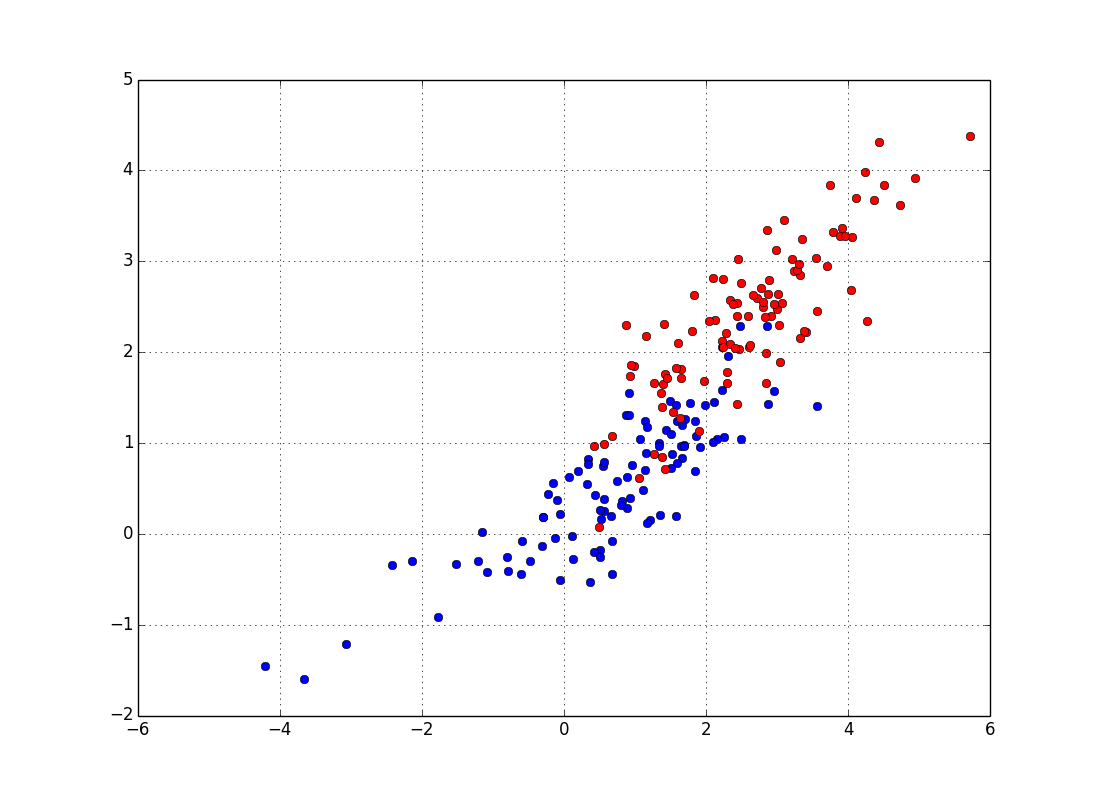
\includegraphics[scale=0.55, trim=0mm 0mm 0mm 0mm, clip=True]{pics/cecha_toz_2.png}
\caption{Rozkład cech dla dwóch najlepszych kanałów dla sygnałów target (czerwony) i non-target (niebieski) przy dwóch uśrednionych realizacjach.}
\label{cecha_toz_2}
\end{figure}

\begin{figure}[H]
\centering
\includegraphics[scale=0.37, trim=57mm 30mm 30mm 15mm, clip=True]{pics/sygnal_toz_4.png}
\caption{Wykres sygnałów target (czerwony) i non-target (niebieski) dla dwóch najlepszych kanałów przy czterech uśrednionych realizacjach.}
\label{sygnal_toz_4}
\end{figure}

\begin{figure}[H]
\centering
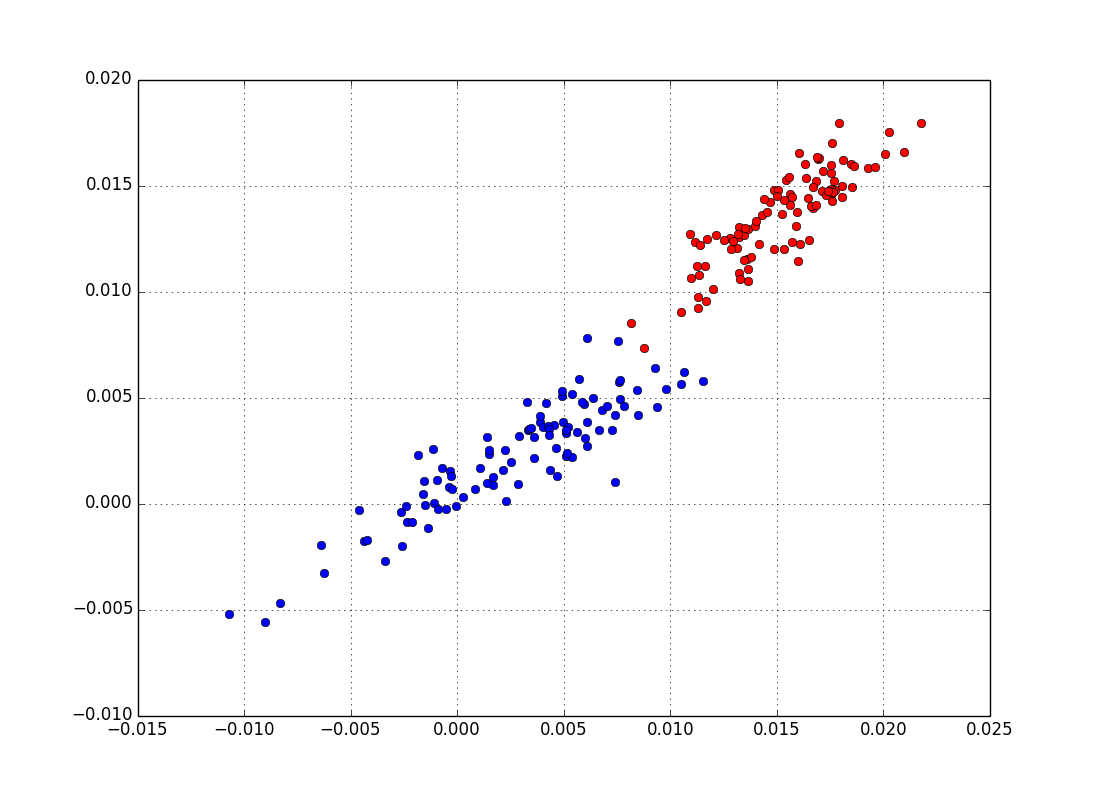
\includegraphics[scale=0.55, trim=0mm 0mm 0mm 0mm, clip=True]{pics/cecha_toz_4.png}
\caption{Rozkład cech dla dwóch najlepszych kanałów dla sygnałów target (czerwony) i non-target (niebieski) przy czterech uśrednionych realizacjach.}
\label{cecha_toz_4}
\end{figure}

\begin{figure}[H]
\centering
\includegraphics[scale=0.37, trim=57mm 30mm 30mm 15mm, clip=True]{pics/sygnal_toz_10.png}
\caption{Wykres sygnałów target (czerwony) i non-target (niebieski) dla dwóch najlepszych kanałów przy dziesięciu uśrednionych realizacjach.}
\label{sygnal_toz_10}
\end{figure}

\begin{figure}[H]
\centering
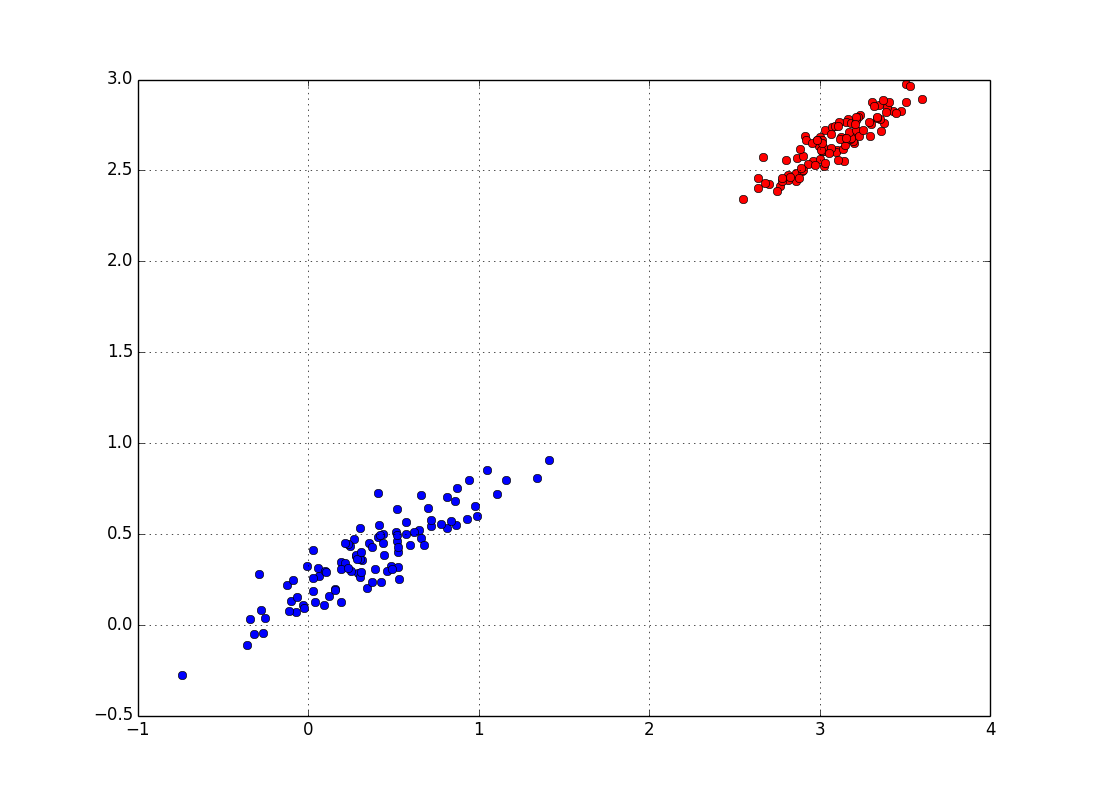
\includegraphics[scale=0.55, trim=0mm 0mm 0mm 0mm, clip=True]{pics/cecha_toz_10.png}
\caption{Rozkład cech dla dwóch najlepszych kanałów dla sygnałów target (czerwony) i non-target (niebieski) przy dziesięciu uśrednionych realizacjach.}
\label{cecha_toz_10}
\end{figure}



\subsection{Transformata Hjorta}

\begin{figure}[H]
\centering
\includegraphics[scale=0.37, trim=57mm 30mm 30mm 15mm, clip=True]{pics/sygnal_hjorth_2.png}
\caption{Wykres sygnałów target (czerwony) i non-target (niebieski dla dwóch najlepszych kanałów przy dwóch uśrednionych realizacjach.}
\label{sygnal_hjorth_2}
\end{figure}

\begin{figure}[H]
\centering
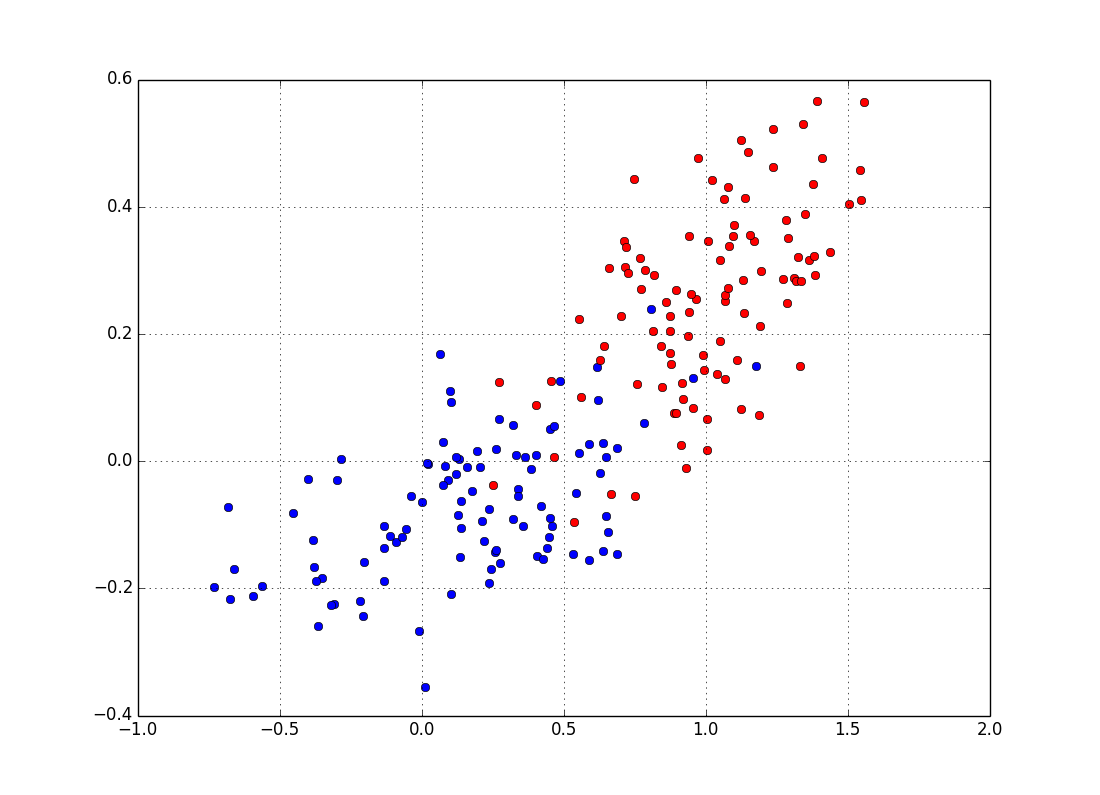
\includegraphics[scale=0.55, trim=0mm 0mm 0mm 0mm, clip=True]{pics/cecha_hjorth_2.png}
\caption{Rozkład cech dla dwóch najlepszych kanałów dla sygnałów target (czerwony) i non-target (niebieski) przy dwóch uśrednionych realizacjach.}
\label{cecha_hjorth_2}
\end{figure}

\begin{figure}[H]
\centering
\includegraphics[scale=0.37, trim=57mm 30mm 30mm 15mm, clip=True]{pics/sygnal_hjorth_4.png}
\caption{Wykres sygnałów target (czerwony) i non-target (niebieski) dla dwóch najlepszych kanałów przy czterech uśrednionych realizacjach.}
\label{sygnal_hjorth_4}
\end{figure}

\begin{figure}[H]
\centering
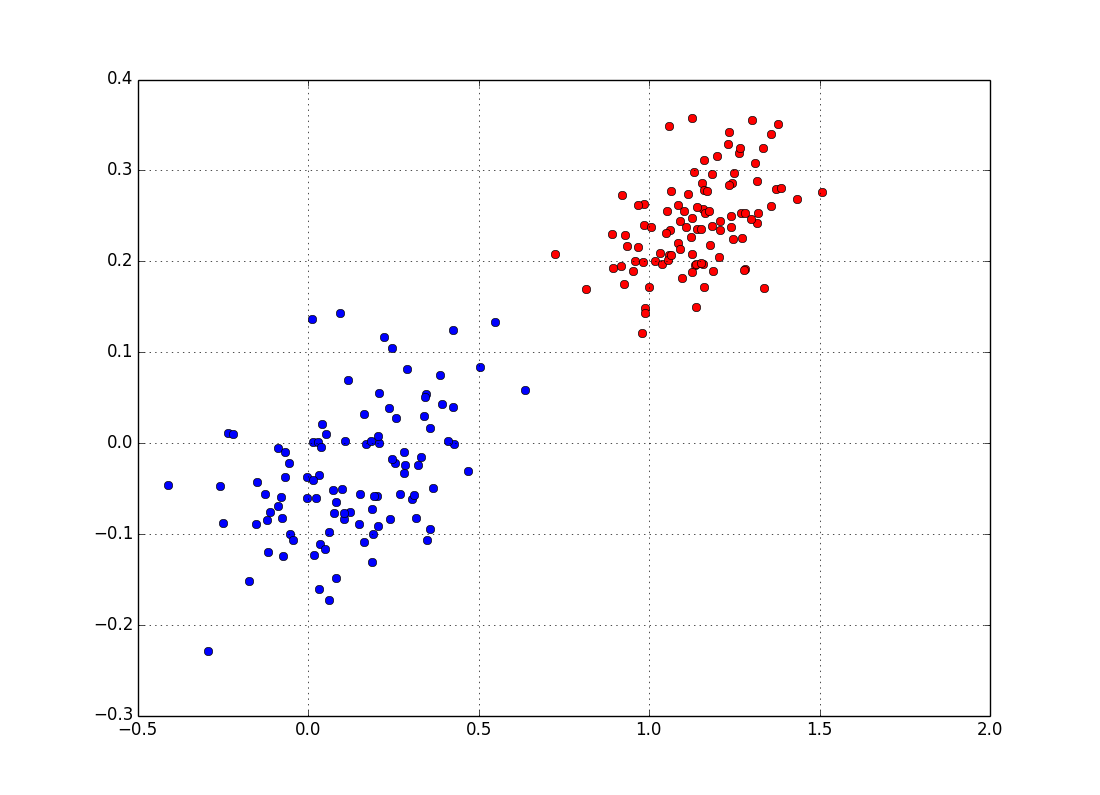
\includegraphics[scale=0.55, trim=0mm 0mm 0mm 0mm, clip=True]{pics/cecha_hjorth_4.png}
\caption{Rozkład cech dla dwóch najlepszych kanałów dla sygnałów target (czerwony) i non-target (niebieski) przy czterech uśrednionych realizacjach.}
\label{cecha_hjorth_4}
\end{figure}

\begin{figure}[H]
\centering
\includegraphics[scale=0.37, trim=57mm 30mm 30mm 15mm, clip=True]{pics/sygnal_hjorth_10.png}
\caption{Wykres sygnałów target (czerwony) i non-target (niebieski) dla dwóch najlepszych kanałów przy dziesięciu uśrednionych realizacjach.}
\label{sygnal_hjorth_10}
\end{figure}

\begin{figure}[H]
\centering
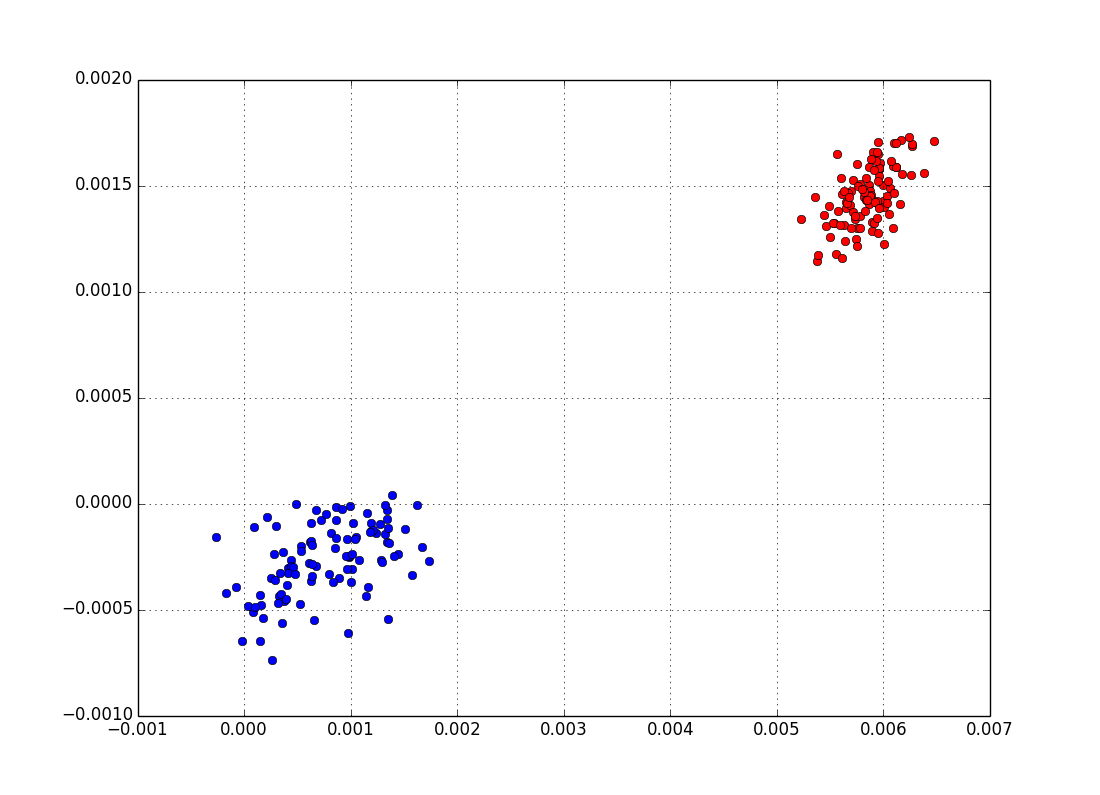
\includegraphics[scale=0.55, trim=0mm 0mm 0mm 0mm, clip=True]{pics/cecha_hjorth_10.png}
\caption{Rozkład cech dla dwóch najlepszych kanałów dla sygnałów target (czerwony) i non-target (niebieski) przy dziesięciu uśrednionych realizacjach.}
\label{cecha_hjorth_10}
\end{figure}


\subsection{Wspólny wzorzec przestrzenny}

\begin{figure}[H]
\centering
\includegraphics[scale=0.37, trim=57mm 30mm 30mm 15mm, clip=True]{pics/sygnal_csp_2.png}
\caption{Wykres sygnałów target (czerwony) i non-target (niebieski) dla dwóch najlepszych kanałów przy dwóch uśrednionych realizacjach.}
\label{sygnal_csp_2}
\end{figure}

\begin{figure}[H]
\centering
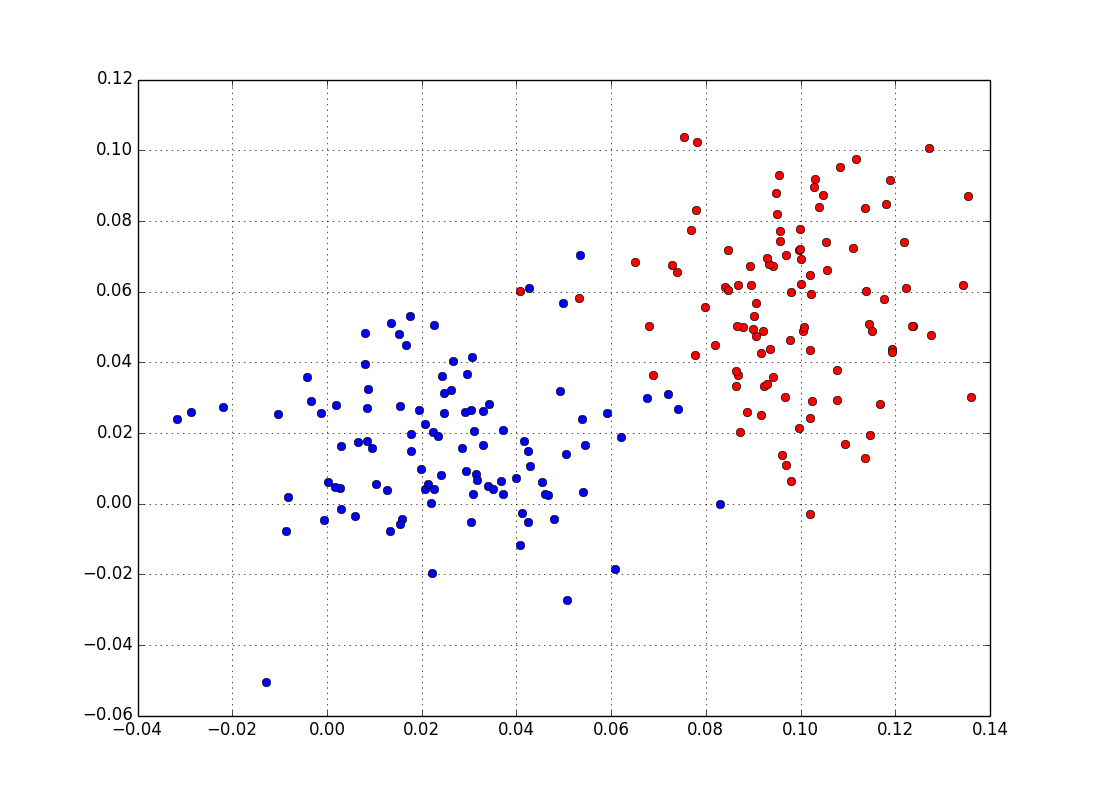
\includegraphics[scale=0.55, trim=0mm 0mm 0mm 0mm, clip=True]{pics/cecha_csp_2.png}
\caption{Rozkład cech dla dwóch najlepszych kanałów dla sygnałów target (czerwony) i non-target (niebieski) przy dwóch uśrednionych realizacjach.}
\label{cecha_csp_2}
\end{figure}


\begin{figure}[H]
\centering
\includegraphics[scale=0.37, trim=57mm 30mm 30mm 15mm, clip=True]{pics/sygnal_csp_4.png}
\caption{Wykres sygnałów target (czerwony) i non-target (niebieski) dla dwóch najlepszych kanałów przy czterech uśrednionych realizacjach.}
\label{sygnal_csp_4}
\end{figure}

\begin{figure}[H]
\centering
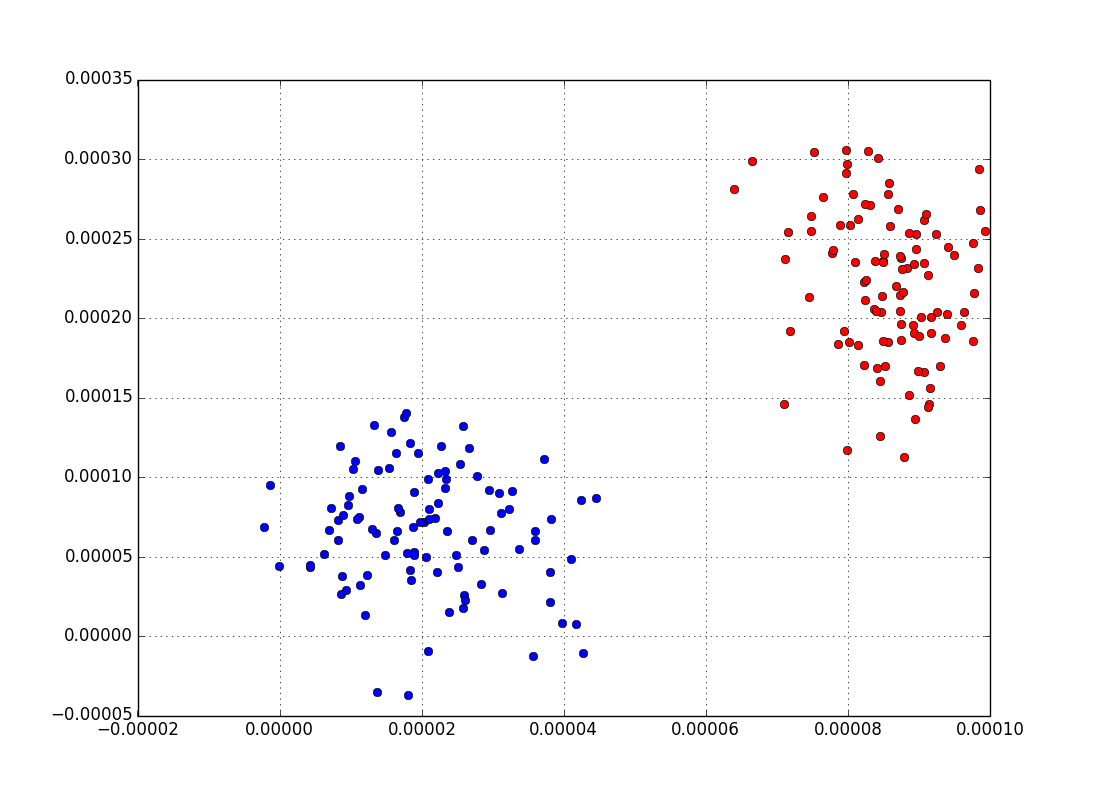
\includegraphics[scale=0.55, trim=0mm 0mm 0mm 0mm, clip=True]{pics/cecha_csp_4.png}
\caption{Rozkład cech dla dwóch najlepszych kanałów dla sygnałów target (czerwony) i non-target (niebieski) przy czterech uśrednionych realizacjach.}
\label{cecha_csp_4}
\end{figure}

\begin{figure}[H]
\centering
\includegraphics[scale=0.37, trim=57mm 30mm 30mm 15mm, clip=True]{pics/sygnal_csp_10.png}
\caption{Wykres sygnałów target (czerwony) i non-target (niebieski) dla dwóch najlepszych kanałów przy dziesięciu uśrednionych realizacjach.}
\label{sygnal_csp_10}
\end{figure}

\begin{figure}[H]
\centering
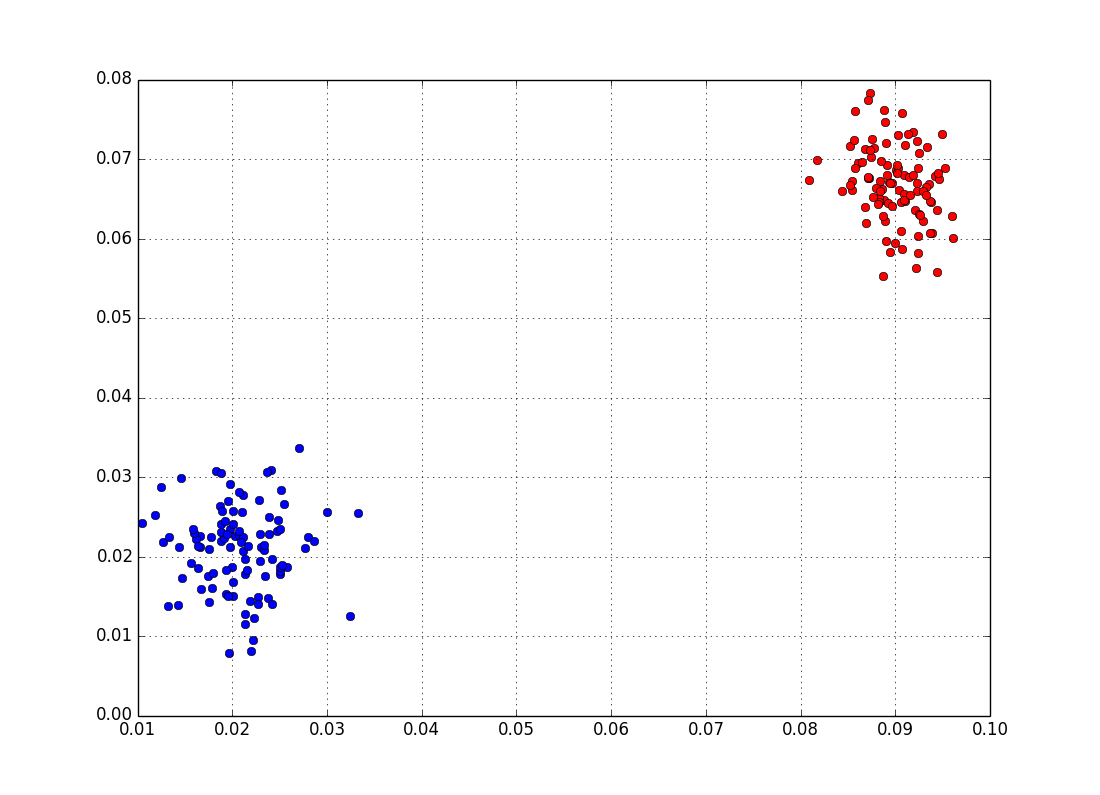
\includegraphics[scale=0.55, trim=0mm 0mm 0mm 0mm, clip=True]{pics/cecha_csp_10.png}
\caption{Rozkład cech dla dwóch najlepszych kanałów dla sygnałów target (czerwony) i non-target (niebieski) przy dziesięciu uśrednionych realizacjach.}
\label{cecha_csp_10}
\end{figure}


\section{Odległość Mahalanobisa}
\begin{figure}[H]
\centering
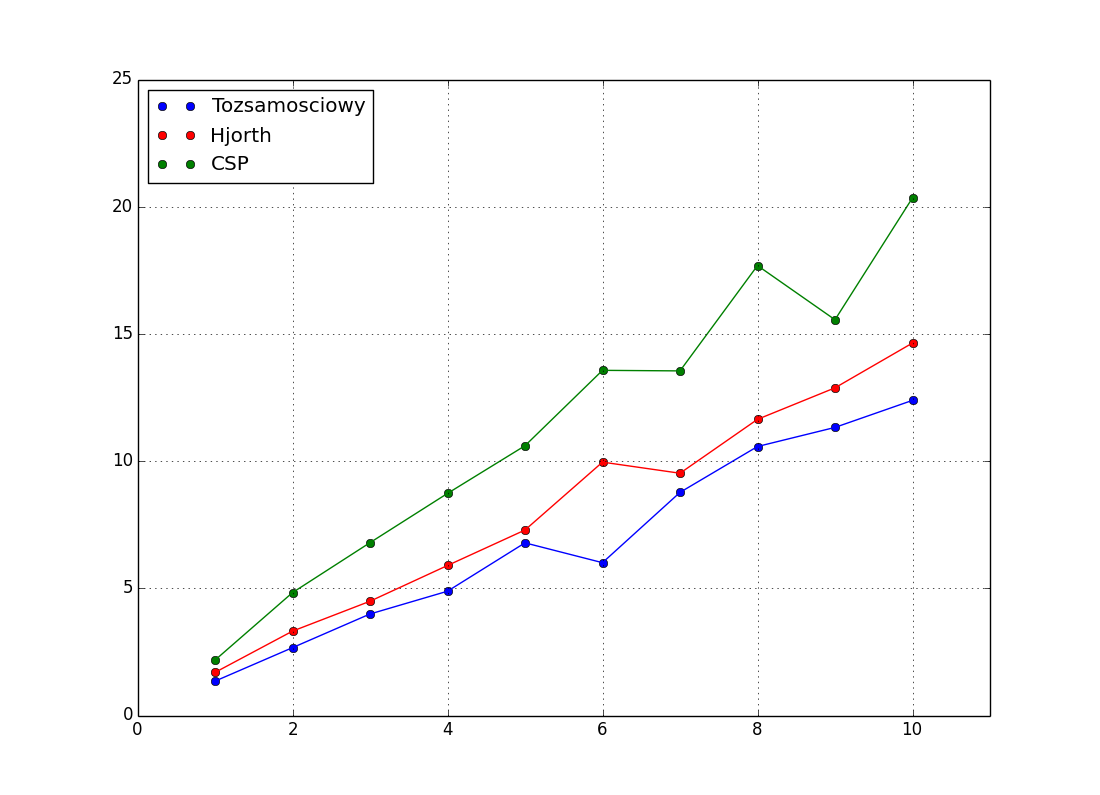
\includegraphics[scale=0.37, trim=57mm 30mm 30mm 15mm, clip=True]{pics/mahalanobis.png}
\caption{Zależność odległości Mahalanobisa od liczby uśrednianych realizacji dla każdego prezentowanego filtru.}
\label{mahalanobis_pic}
\end{figure}

\todo[inline]{tu komentarz, że wszystko zgodnie z oczekiwaniami, najlepsze csp, potem hjorth i tozsamosciowy}


\chapter{Dyskusja i Wnioski}
\todo[inline]{Mam problem, bo Machalanobis robi dziwne rzeczy. Bierze kanały niekoniecznie optycznie najlepsze. W CSP wymusiłem, żeby brał 1 i 0. Ale w reszcie bierze to co daje najlepszy wynik i czasami są to kanały nie intuicyjne. Tak jak na rysunku \ref{sygnal_toz_2} i \ref{cecha_toz_2} wziął sobie O1 i O2, w których nic nie ma. Mam mu wymusić branie jakiś dwóch konkretnych kanałów? Mam wszystko oskryptowane, więc to kwestia podmienienia zmiennej na numer kanału.

Drugim problemem jaki mam to transformata Hjorta. Wszystko działa tak jak oczekuje, wyniki są lepsze, niż surowego sygnału (rys. \ref{mahalanobis_pic}), ale optycznie to dziwnie wygląda.

Jutro będę na Hożej od 10 jakoś i zostaje dopóki nie skończę. Mam nadzieję, że to już ostatnia prosta.}


\bibliography{biblio}
\end{document}
